\documentclass{article}

\usepackage{dirtree}

\usepackage[
  height=9in,      % height of the text block
  width=7.5in,       % width of the text block
  top=78pt,        % distance of the text block from the top of the page
  headheight=48pt, % height for the header block
  headsep=12pt,    % distance from the header block to the text block
  heightrounded,   % ensure an integer number of lines
        % show the main blocks
  verbose,         % show the values of the parameters in the log file
]{geometry}
\setlength{\parindent}{0pt}
\usepackage{amsmath}
\usepackage{courier}
\usepackage{graphicx}
\usepackage{amsmath}
\usepackage{booktabs}
\usepackage{fancyhdr}
\usepackage{float}
\usepackage{mathtools}

\pagestyle{fancy}
\fancyhead[L]{Pattern and Speech Recognition WS1617\\ Assignment 05}
\fancyhead[R]{ Vinh Thinh Ho (2562630) \\ Noshaba Cheema (2562653)}



\renewcommand{\headrulewidth}{0.4pt}
\newcommand\tab[1][1cm]{\hspace*{#1}}

\begin{document}
\section*{Exercise 5.1}
a)\\
With $ReLU(z) = max(0,z)$:
\begin{align*}
\frac{\partial ReLU(z)}{\partial z} = 
\begin{cases}
\frac{\partial 0}{\partial z} = 0\ when\ z \leq 0\\
\frac{\partial z}{\partial z} = 1\ when\ z \geq 0
\end{cases}
\end{align*}
With sigmoid function $g(z) = \frac{1}{1+e^{-z}}$:
\begin{align*}
\frac{\partial g(z)}{z} &= \frac{-1}{(1 + e^{-z})^2}. \frac{\partial (1 + e^{-z})}{\partial z}\\
&= \frac{e^{-z}}{(1 + e^{-z})^2} = \frac{1}{1 + e^{-z}}.\frac{e^{-z}}{1 + e^{-z}}\\
&=g(z).(1-g(z)) = g(z).g(-z)
\end{align*}
b)
We can see that the value of $g'(z)$ can be derived from $g(z)$. Hence, for a given layer that use sigmoid function as activation function, we can just store the value $g(z)$, then the gradient $g'(z)$ of that layer could be evaluated directly from $g(z)$ by simple multiplication and subtraction.
\section*{Exercise 5.2}
See \textbf{nn.py}\\
We use sigmoid activation function in the hidden layer only, and linear activation in output layer. In addition the dimension for hidden layer is 256. We trained the model with 30 epochs and learning rate 0.05

Below is the graph of MSE loss function after each epoch and accuracy after each epoch (training process uses MNIST train data and accuracy is evaluated basing on MNIST test data)

\begin{figure}[H]
	\centering
	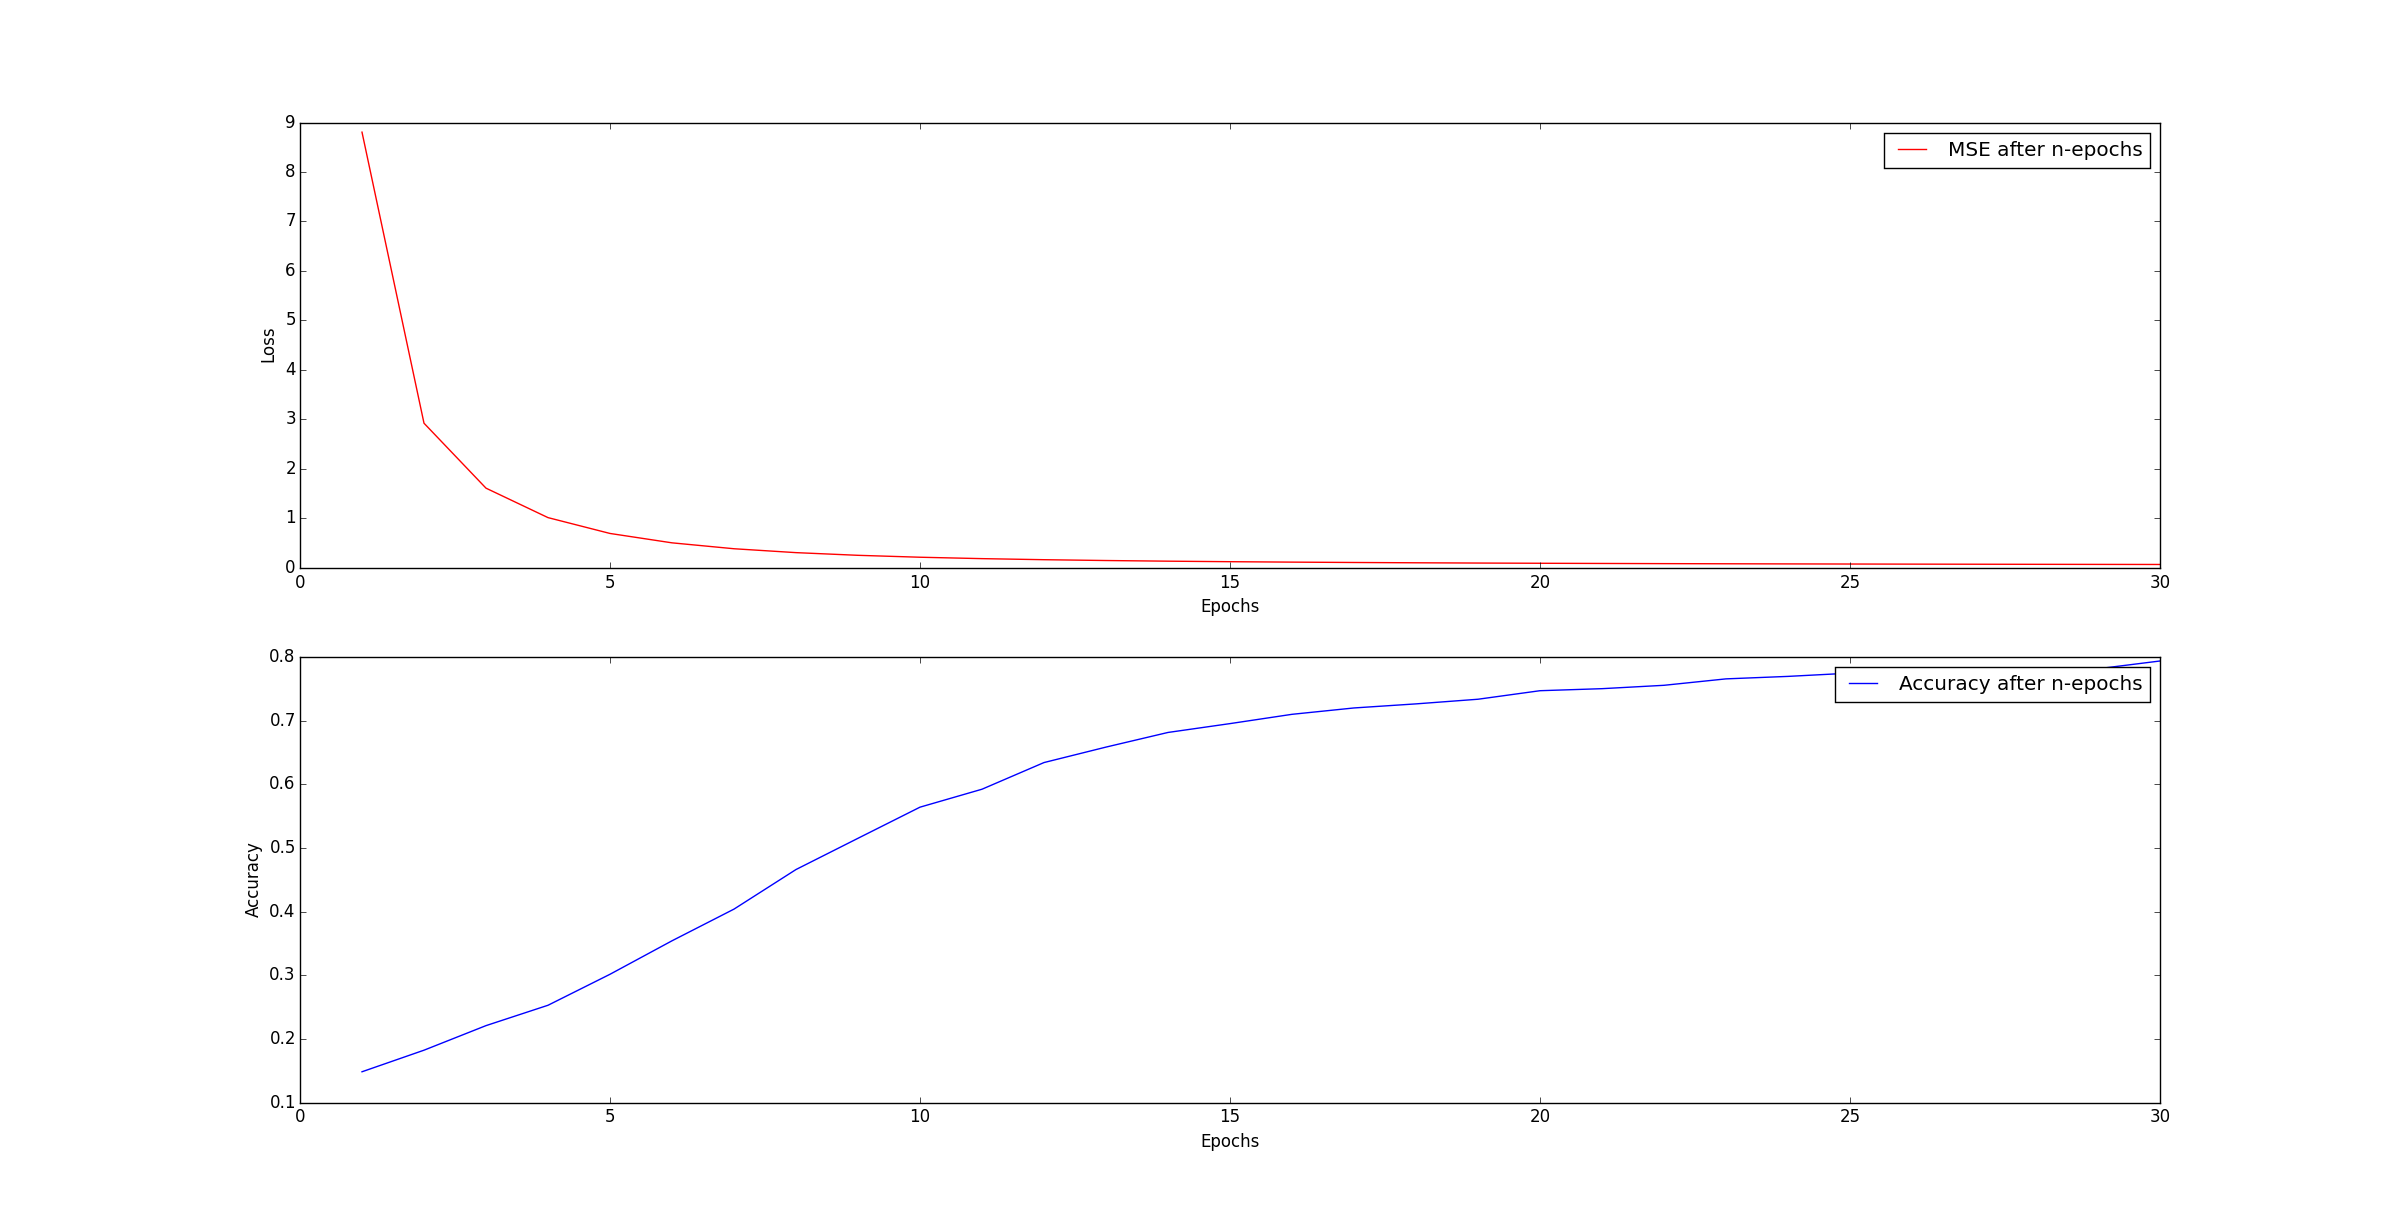
\includegraphics[scale=0.3]{nn.png}
	\caption{Classification Result}
	\label{fig3}	
\end{figure}
\end{document}



